\chapter{Antecedentes}

En este capítulo se discuten los antecedentes y el marco teórico necesario para poder entender este trabajo. Además, se muestran las definiciones formales utilizadas en el resto del documento.

\section{Information flow control}

	La protección de la confidencialidad de la información manipulada por los programas computacionales es un problema cuya relevancia se ha incrementado en el último tiempo, a pesar de tener varias décadas de investigación. Por ejemplo, una aplicación web (o móvil) que como parte de su funcionamiento debe interactuar con servicios de terceros y por tanto debe proteger que su información sensible no se escape durante la ejecución de la aplicación a canales públicos.

	Muchas de las técnicas de seguridad convencionales como \textit{control de acceso} tienen deficiencias para proteger la confidencialidad de un programa, por ejemplo no restringen la propagación de información\cite{myers-phd}.% TODO citation needed

	Un mecanismo más expresivo para la protección de la confidencialidad e integridad de la información se denomina \textit{information flow control}. Mientras control de acceso restringe qué datos pueden ser accedidos, \textit{information flow control} restringe el flujo de estos datos.

	\subsection{Tipado de seguridad}
	El análisis de \textit{information flow control} puede ser realizado sobre el código del programa, de forma estática o dinámica. Una de las técnicas más efectivas de \textit{information flow control} con análisis estático es \textit{tipado de seguridad} en un \textit{lenguaje de seguridad}. En un lenguaje de seguridad, los valores y los tipos son anotados con niveles de seguridad para clasificar la información que el programa manipula. Dichos niveles de seguridad forman una \textit{lattice}\footnote{Un orden parcial, donde todo par de elementos tiene un único supremo e ínfimo}.

	\begin{figure}[ht]
		\centering
		\begin{tikzpicture}
			\node(H) 												{$H$};
			\node(L)      [below of=H]       {$L$};
			\draw(H)      -- (L);
		\end{tikzpicture}
		\caption{\textit{lattice} de dos niveles de seguridad}
	\end{figure}


	Por ejemplo con la \textit{lattice} de dos niveles de seguridad $L \sqsubseteq H$, se puede distinguir entre valores enteros públicos o de baja confidencialidad ($Int_L$) y valores enteros privados o de alta confidencialidad ($Int_H$). El sistema de tipos usa estos niveles de seguridad para prevenir que la información confidencial no fluya directa o indirectamente hacia canales públicos\cite{volpanoAl:S96}. % TODO citation needed

	\begin{lstlisting}
String @H login(String @L guess, String @H password) {
	if (password == login) return "Login successful";
	else return "Login failed";
}
	\end{lstlisting}

	En el código anterior, los tipos de los parámetros y el tipo de retorno de la función están etiquetados con niveles de seguridad. En este ejemplo, la operación \texttt{password == login} tiene un nivel de seguridad \texttt{@H}, debido a que las operaciones binarias tienen un nivel de seguridad que corresponde a la operación \texttt{join} en la \textit{lattice} a la cual pertenecen los elementos. Como el nivel de seguridad se propaga desde la condición del \texttt{if} hacia ambas ramas, el tipo de retorno de la función también tiene un nivel de seguridad \texttt{@H}.

	\subsection{Flujo explícito}
	Se denomina flujo explícito a las instrucciones del programa que directamente asignan un valor a una variable con distintos niveles de seguridad. El siguiente programa ilustra el flujo explícito.

	\begin{lstlisting}
void @L foo(int @H highVar, int @L lowVar) {
		int @H v1 = lowVar;
		int @L v2 = highVar;
}
	\end{lstlisting}

	En el ejemplo, la primera asignación no representa un riesgo de seguridad, puesto que se asigna un valor público a una variable confidencial. Por otra parte, la segunda asignación es insegura, debido a que se asigna un valor confidencial a una variable pública, que luego puede ser utilizada en contextos no deseados.

	\subsection{Flujo implícito}

	Se denomina flujo implícito a las instrucciones del programa que indirectamente dan conocimiento de algún aspecto de una variable, usualmente mediante instrucciones condicionales. Podemos adaptar el mismo programa de \texttt{login} visto anteriormente para ilustrar el flujo implícito.

	\begin{lstlisting}
String @L login(String @L guess, String @H password) {
	String @L ret;
	if (password == login) ret = "Login successful";
	else ret = "Login failed";
	return ret;
}
	\end{lstlisting}

	En este ejemplo, las instrucciones de asignación a la variable \texttt{ret} son seguras por si solas, pero no lo son considerando que su ejecución depende del valor de una variable confidencial, en este caso \texttt{password}.

	\subsection{No-interferencia}
	La propiedad para formalizar y caracterizar la seguridad y confidencialidad en los lenguajes con tipado de seguridad se denomina \textit{no-interferencia (noninterference)}. A grandes rasgos noninterference expresa que para dos ejecuciones realizadas por el adversario de un programa seguro, con valores confidenciales equivalentes, las salidas del programa deben ser equivalentes para el adversario. Esto caracteriza que el adversario no aprende nada sobre los valores confidenciales de un programa.

	El programa de \texttt{login} es un buen ejemplo para ilustrar el concepto de noninterference.

	\begin{lstlisting}
String @H login(String @L guess, String @H password) {
	if (password == login) return "Login successful";
	else return "Login failed";
}
	\end{lstlisting}

	Este programa no cumple con noninterference, debido a que el adversario puede aprender sobre la variable confidencial \texttt{password} observando el valor de retorno del método para distintas ejecuciones.

	\subsection{Declasificación}
	En una aplicación real y práctica deseamos que el programa anterior sea aceptado a pesar de violar la propiedad de no-interferencia, pues de otra forma no tendríamos cómo realizar la autenticación. Para solucionar este problema, los lenguajes de seguridad adicionan mecanismos para \textit{declasificar} la información confidencial, implementados de diferentes formas\cite{sabelfeldSands:JCS09}. Una de ellas, por ejemplo en Jif (un lenguaje de seguridad)\cite{jif} es usar un operador \texttt{declassify}, como se indica en el siguiente ejemplo, declasificando la comparación de igualdad del parámetro confidencial \texttt{password} con el parámetro público \texttt{guess} %TODO citation needed.

\begin{lstlisting}
String login(String password, String guess) {
	if (declassify(password == guess)) return "Login Successful";
	else return "Login failed";
}
\end{lstlisting}

	Esto no corresponde a una amenaza de seguridad, debido a que el resultado de la operación de comparación es negligible con respecto al parámetro privado \texttt{password}. Sin embargo, usos arbitrarios del operador \texttt{declassify} pueden resultar en serias fugas de información, como por ejemplo \texttt{declassify(password)}.

	\section{Type-based declassification}

	Varios mecanismos se han explorado para controlar el uso de declasificación, y poder asegurar además una propiedad de seguridad para el programa\cite{sabelfeldSands:JCS09}. En esta dirección, Cruz et al.\cite{cruzAl:ecoop2017} recientemente propusieron \textit{type-based declassification} como un mecanismo de declasificación que conecta la abstracción de tipos con una forma controlada de declasificación, en una manera intuitiva y expresiva, proveyendo garantías formales sobre la seguridad del programa. %TODO citation needed.

	\subsection{Sistema de tipos}

	En \textit{type-based declassification} los tipos tienen dos facetas, una que refleja el tipo de implementación y otro tipo que refleja las operaciones de declasificación sobre los valores de dicho tipo. Por ejemplo, el tipo $\text{StringEq} \triangleq [\text{eq} : \text{String} \rightarrow \text{Bool}]$ autoriza la operación \texttt{eq} sobre un String. Entonces se puede usar el tipo de dos facetas $\text{String} < \text{StringEq}$, en donde String es un subtipo de StringEq, para controlar la operación de declasificación de la igualdad sobre \texttt{password}.

	\clearpage

	\begin{lstlisting}
String login(String<StringEq password, String guess) {
	if (password.eq(guess)) return "Login successful";
	else return "Login failed";
}
	\end{lstlisting}

	Al igual que en tipado de seguridad con etiquetas (@L y @H), la faceta de declasificación es parte de la jerarquía de tipos, la que forma una \textit{lattice} como se muestra en la figura siguiente.

	\begin{figure}[ht]
		\centering
		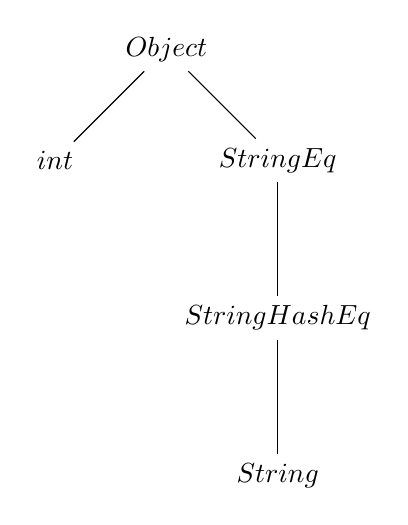
\begin{tikzpicture}[node distance=2cm]
			\node(Object) 												{$Object$};
			\node(StringEq)		[below right of=Object]			{$StringEq$};
			\node(StringHashEq)      [below of=StringEq]       {$StringHashEq$};
			\node(String)				[below of=StringHashEq]       {$String$};
			\node(int)					[below left of=Object] 			{$int$};
			\draw(Object)      -- (StringEq);
			\draw(Object)      -- (int);
			\draw(StringEq)      -- (StringHashEq);
			\draw(StringHashEq)      -- (String);
		\end{tikzpicture}
		\caption{\textit{lattice} de tipos de dos facetas}
	\end{figure}

	De la misma forma, el tipo de las operaciones binarias se resuelve utilizando el operador \texttt{join} sobre la \textit{lattice}.

	\subsection{Formalización}

	Para formalizar y demostrar propiedades del sistema de tipos, se utilizó el lenguaje $\text{Ob}_{\text{SEC}}$, que se muestra en la figura.

	\begin{figure}[ht]
		\centering
		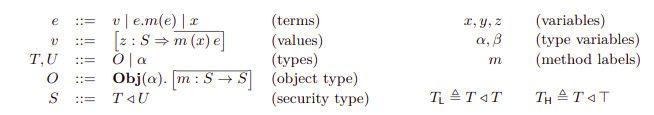
\includegraphics[scale=0.7]{imagenes/obsec.png}
		\caption{Sintaxis de $\text{Ob}_{\text{SEC}}$}
		\label{}
	\end{figure}

	$\text{Ob}_{\text{SEC}}$ es un lenguaje minimalista, y por tanto no soporta características comunes de lenguajes de programación, como asignaciones a variables y condicionales. La justificación de su uso se debe a que es suficiente para formular y demostrar la proposición.

	\subsubsection{Type Safety}

	Se demostró que programas de $\text{Ob}_{\text{SEC}}$ bien tipados son \textit{safe}\footnote{Sin errores de tipos en tiempo de ejecución}.

	\subsubsection{Relaxed noninterference}

	La propiedad de seguridad que se demuestra para $\text{Ob}_{\text{SEC}}$ es una forma de no-interferencia con políticas de declasificación, denominada \textit{Relaxed noninterference}.	Un lenguaje de seguridad que tiene esta propiedad, garantiza que la información confidencial solo puede fluir hacia canales públicos de una forma controlada, por medio de las políticas de declasificación\cite{cruzAl:ecoop2017}.

	\section{Inferencia de tipos de seguridad}

	La inferencia de tipos se refiere a la detección automática del tipo de una expresión en un lenguaje de programación. En \textit{Security Typing}, las expresiones también poseen un tipo de seguridad, el cual puede estar implícito o no especificado, por lo que es posible desarrollar un algoritmo de inferencia para tipos de seguridad.

	En esta dirección, se han desarrollado modelos de inferencia de tipos de seguridad, para lenguajes orientados a objetos\cite{SunBanerjeeGiacobazzi} y lenguajes funcionales\cite{Pottier}, con el objetivo de extender los modelos simplificados para los cuales se demuestran las propiedades de seguridad relevantes.

	Para llevar registro del nivel de seguridad en cada instrucción del programa, se utiliza el concepto de \textit{program counter} (PC) para seguridad\cite{Molnar:2005}. Este registro es utilizado por los modelos de inferencia de tipos de seguridad, y para realizar el análisis de seguridad que detecta la existencia de fugas de información.

	\section{Lenguaje Dart}

	Dart es un lenguaje de programación de propósito general, orientado a objetos y de código abierto desarrollado por Google. Es usado para construir aplicaciones web, móviles y dispositivos IoT (Internet of Things). % TODO citation needed

	Dart es un lenguaje de creciente adopción. Actualmente, la interfaz de Google Adwords está construida sobre Dart y Angular2. Además, Dart es usado en el framework de desarollo multiplataforma \textit{Flutter}.

	El lenguaje Dart fue escogido porque los investigadores que realizaron el trabajo de \textit{type-based declassification} estudian este lenguaje como parte de un proyecto de investigación mayor en el área de seguridad. Es factible implementar el enfoque de \textit{type-based declassification} en Dart, dado que fue formalizado considerando un lenguaje minimalista orientado a objetos ($\text{Ob}_{\text{SEC}}$).

	Se utilizaron de forma intensiva dos librerías en el desarrollo de este trabajo.

	\subsection{Dart Analyzer}

	La herramienta \textit{Dart Analyzer} sirve para realizar análisis estático de código Dart. Al usarse como librería, se puede obtener el \textit{Abstract Syntax Tree} (AST)\footnote{Representación de árbol de la estructura sintáctica abstracta del código fuente} del código, el cual contiene, en sus nodos, la información de los distintos elementos que conforman la sintaxis, y también la inferencia de tipos resuelta. % TODO citation needed

	Por ejemplo, para el siguiente código en Dart

	\begin{lstlisting}
class Bar {
	inf foo(int a) {
		var b = 2*a;
		return b;
	}
}
	\end{lstlisting}

	Dart Analyzer genera el siguiente AST, en donde se indica el tipo de nodo y la expresión al cual corresponde

	\clearpage

	\begin{figure}[ht]
		\centering
		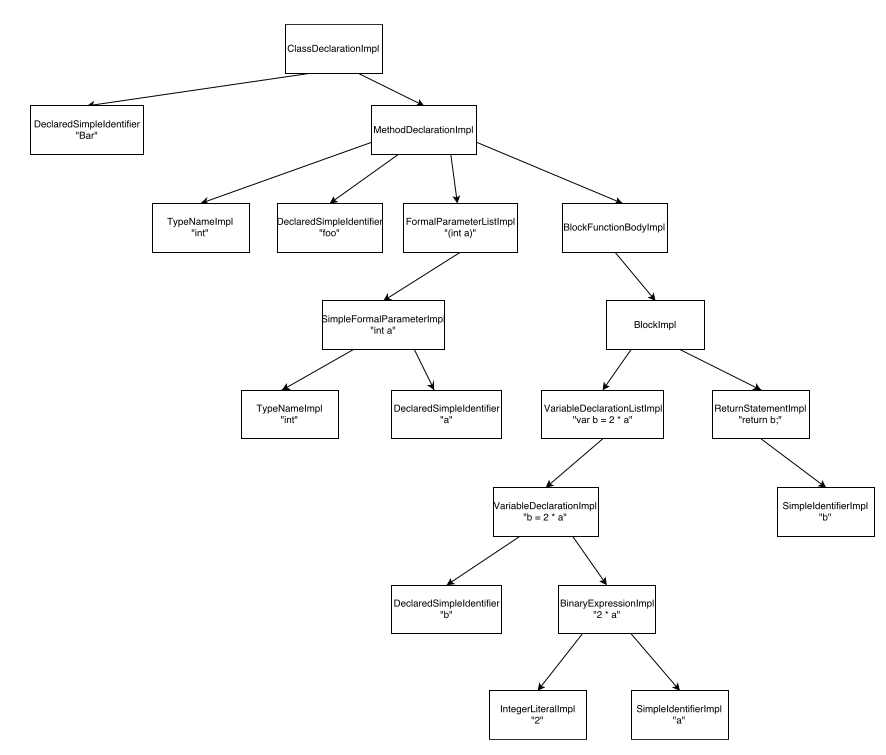
\includegraphics[scale=0.58]{imagenes/ast.png}
		\caption{Representación del AST generado por Dart Analyzer}
		\label{}
	\end{figure}

	Con Dart Analyzer es posible realizar análisis personalizado sobre el AST, utilizando el patrón de diseño \textit{Visitor}.

	\subsection{Analyzer Plugin}

	La herramienta \textit{Analyzer Plugin} sirve para integrar un análisis personalizado sobre el AST generado por \textit{Dart Analyzer} con los editores de texto más populares, como IntelliJ, Eclipse, Atom, entre otros. Con esta librería es posible mostrar errores, \textit{warnings}, sugerencias de edición y resaltado de sintaxis. % TODO citation needed
